\subsubsection{Minimizando el error}\label{minimizing-error}

Una vez elegida alguna de las funciones de coste, el objetivo es minimizar el error y así mejorar el modelo:

\begin{equation}
\begin{split}
        W^* &= \argmin_{W} \frac{1}{n} \sum_{i=1}^n c(a(x^{(i)}; W), y^{(i)}) \\
        &= \argmin_{W} c_i(W) \\
        \text{donde}~x^{(i)} &= \text{Vector de entrada para el dato }i \\
        y^{(i)} &= \text{Vector real para el dato }i \\
        W &= \text{Matrices con los pesos y bias de cada cada} 
  \end{split}
\end{equation}

Para calcular el mínimo de una función, se necesita calcular la derivada de dicha función e igualarla a $0$. Minimizando la función de coste, es decir, derivando la función de coste, también se minimiza el error. Para ello hay distintas formas de minimizar el error:
\begin{itemize}
\item Minimizar función de coste

Este fue el algoritmo usado en las redes de perceptrones para calcular la matriz $W$. El funcionamiento de este algoritmo es sencillo. Partiendo de la definición de una función de coste cualesquiera que permita cuantificar el error del modelo, se tratará de minimizar dicho valor. Una de las ecuaciones más populares es la que se conoce como el \acrlong{ols}. Esta función parte de la derivada de \acrshort{mse}:

\begin{equation}
    \begin{split}
    L_i & =  (\hat{y_i} - y_i)^2 \\
     & = (y - x \cdot W)' \cdot (y - x \cdot W) \\
     & = y'y - W'x'y - y'xW + W'x'x W
  \end{split}
\end{equation}

Derivando y despejando:
\begin{equation}
    \begin{split}
L_i'() = & -2x'y + 2x'xW \\
W^* = & (x'x)^{-1}x'y
\end{split}
\end{equation}

Esta ecuación permite el cálculo de la matriz $W$ óptima posible solo usando los valores de entrada y de salida de modelo como argumentos. Aunque este algoritmo de entrenamiento tiene varias limitaciones:
\begin{itemize}
\item No es extensible a redes más complejas.
\item El cálculo de la matriz inversa es muy costoso computacionalmente.
\item Se ha usado el error mínimo cuadrado, una de las más simple, puesto que es una función con forma convexa y por tanto una derivada fácil de calcular, pero hay otras funciones de coste que no permiten minimizar el error con esta técnica.
\newline

Estas limitaciones, demostradas matemáticamente en el libro "\textit{Perceptron}"\cite{papert} de Minsky y Papert (1969), provocó un corte repentino en la financiación de proyectos de inteligencia artificial y más específicamente en aquellos relacionados con los sistemas de redes neuronales durante un periodo de más de 15 años conocidos como el invierno de la inteligencia artificial.
\end{itemize}


\item Descenso del gradiente

Este algoritmo no es una fórmula como los mínimos cuadrados ordinarios, sino un método iterativo que poco a poco va minimizando el error. De algún modo se puede asimilar a como aprendemos los seres humanos: No con una única fórmula, sino a través de la experiencia reduciendo nuestros errores con el tiempo.
\newline

El cálculo del gradiente es un proceso que se puede representar de la siguiente forma:
\begin{figure}[H]
    \centering
    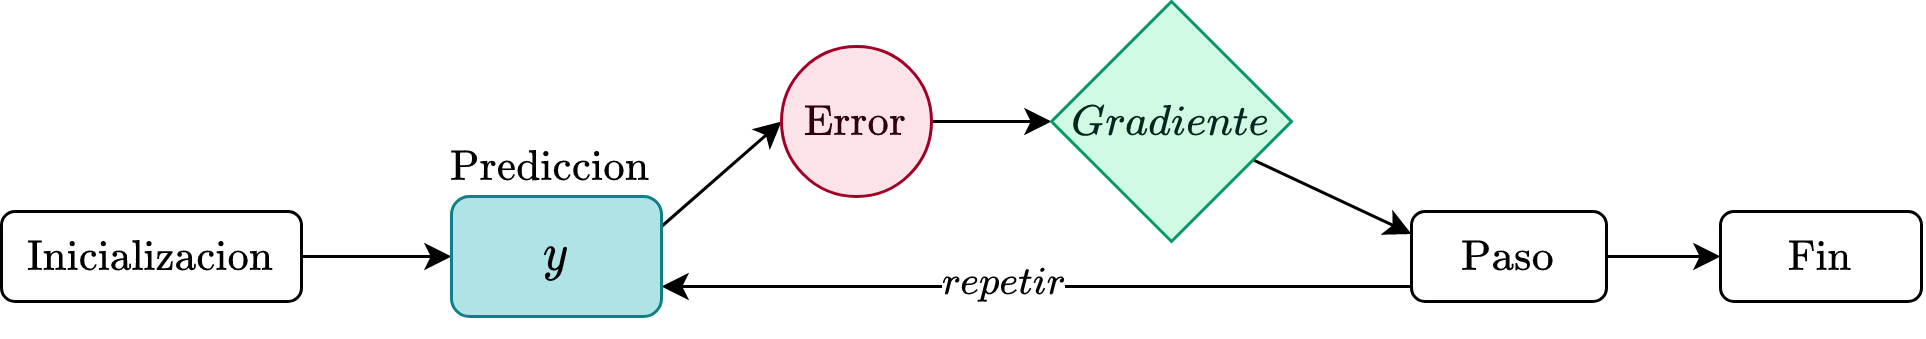
\includegraphics[width=13cm]{images/state-of-art/gradient-descent/gradient-algorithm.png}
    \caption{Proceso iterativo para minimizar el error}
    \label{fig:gradient_descent}
\end{figure}

El método de los \acrshort{ols} minimiza el error igualando la derivada a $0$ para poder hallar los mínimos de \acrshort{mse}. Con esto, se pueden calcular los mínimos locales y globales, pero también se puede calcular máximo locales, puntos de inflexión o puntos de silla provocando un sistema de ecuaciones grande y bastante ineficiente de resolver \cite{papert}.
\newline

Una forma de entender este método es el siguiente: Una persona se encuentra en un terreno montañoso y el objetivo de esta persona es llegar al punto más bajo. Para ello, analizará el terreno donde se encuentra y evaluará la pendiente y se moverá hacia donde la pendiente desciende con mayor intensidad. Descenderá una cantidad de pasos y repetirá el proceso: analizar la inclinación y descender. Esto se repetirá hasta que llegué a lo más abajo posible y no haya forma alguna de seguir bajando. Esta es la lógica del algoritmo del descenso del gradiente.

\begin{figure}[H]
    \centering
    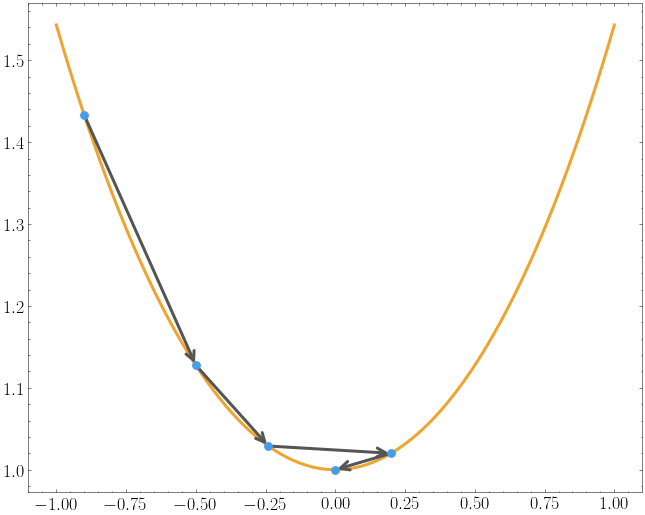
\includegraphics[width=7cm]{images/state-of-art/gradient-descent/gradient.png}
    \caption{Ejemplo gráfico de la iteración del descenso del gradiente}
    \label{fig:gradient_descent}
\end{figure}


El terreno en esta metáfora sería la función de coste. La persona es el valor calculado por la función de coste, el cual se quiere minimizar y por ello se evalúa la pendiente o gradiente solo en ese punto y de ese modo no se depende de la derivada de la función de coste sino de la derivada parcial respecto a cada uno de los valores de entrada en la neurona. El número de pasos que la persona bajará es un valor conocido como tasa de aprendizaje (\textit{learning rate} en inglés) y es un parámetro más de la red neuronal. 
\newline


En la figura \ref{fig:gradient_descent}, hay dos ejes, representando una neurona que tiene solo un argumento de entrada. El eje de ordenadas representa el error de la neurona. Se ha representado un espacio bidimensional, pero se puede usar cualquier dimensión puesto que el número de entradas de la neurona no está limitado. Usando un espacio tridimensional, la función de coste sería una superficie irregular. De hecho, el vector $\nabla f$ siempre tendrá como mínimo dos valores, un peso $w$ y la bias $b$.
\newline

En este trabajo no se explica cómo calcular la derivada de una función o derivada parcial($\sigma$). Dicho esto, matemáticamente, el proceso de este algoritmo es el siguiente \cite{}:
\begin{enumerate}
\item Se inicializa los pesos $w$ y bias $b$ de la neurona quieren ajustar de forma aleatoria:
\begin{equation}
    ~N(0, \sigma_2)
\end{equation}

\item Se realiza un bucle hasta la convergencia:
\begin{enumerate}

\item Se calculan derivadas parciales para cada uno de los parámetros. Una derivada parcial mide cuanto impacto tiene una única variable de entrada en la salida de la función y se calcula igual que una derivada, lo único que se repite la derivada para cada variable de entrada. Cada uno de esos valores indicará cual es la pendiente en el eje de dicho parámetro relacionado a un único valor de entrada.

\begin{equation}
    \begin{split}
    \nabla f &= \nabla f_b \oplus \nabla f_w \\\
    \nabla f_b &= \begin{pmatrix} \frac{\partial c}{\partial b} \end{pmatrix}\\
    \nabla f_w &= \begin{pmatrix} \frac{\partial c}{\partial w_1}, & \frac{\partial c}{\partial w_2}, & \cdots , &  \frac{\partial c}{\partial w_n} \end{pmatrix}
  \end{split}
  \label{eqn:gradients}
\end{equation}


Conjuntamente todas las direcciones, es decir, todas las derivadas parciales conforman un vector que indica la dirección a la que la pendiente asciende, este vector es también conocido como gradiente($\nabla f$) y el cual tendrá el mismo número de elementos que el vector de entrada y cada valor contendrá la solución a la derivada parcial con respecto a cada uno de los valores de entrada.
\newline

El objetivo de esta función es minimizar y no maximizar, por lo que se negará el gradiente para indicar la dirección en la que la pendiente desciende.

\begin{equation}
    \nabla f = -\nabla f_b \oplus \nabla f_w
\end{equation}

\item Se actualizan los pesos con los nuevos valores del gradiente negativo multiplicado por la tasa de aprendizaje. La tasa de aprendizaje es simplemente un valor que determina como de grande será el paso en cada iteración que se verá con mayor profundidad en la sección \ref{learningrate}:
\begin{equation}
    \begin{split}
    b^* = b - \eta * \nabla f_b \\
    w^* = w - \eta * \nabla f_w
    \end{split}
\end{equation}

Al igual que ocurría con el algoritmo de \textit{feed-forward}, el descenso del gradiente trabajará por capas, por lo que este último paso se debería representar de la siguiente forma:

\begin{equation}
    W^* = W - \eta * \nabla f
\end{equation}

Esta ecuación representa que se actualizarán los pesos de todas las neuronas en una capa.

\end{enumerate}
\end{enumerate}

Este método se aplicará a todas las neuronas de la red. Dado un error, el descenso del gradiente obtendrá un vector que contendrá la derivada de los parámetros respecto al coste. Es decir, el gradiente será un vector con distintos valores, cuanto más grande sea dicho valor, más corrección se debe aplicar al parámetro que corresponde. Visto gráficamente se puede ver de la siguiente forma:

\begin{figure}[H]
    \centering
    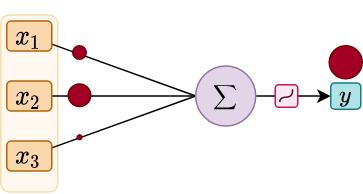
\includegraphics[width=7cm]{images/state-of-art/gradient-descent/gradient_diagram.png}
    \caption{Representación del descenso del gradiente en una neurona. Lo rojo es la representación del error.}
    \label{fig:gradient_descent}
\end{figure}

Las derivadas parciales que se deben resolver para obtener el vector gradiente $\nabla f$, indica como varía el coste ante el cambio de los parámetro $w$ y $b$. A continuación, se muestra una imagen de las distintas partes de las derivadas parciales:

\begin{figure}[H]
    \centering
    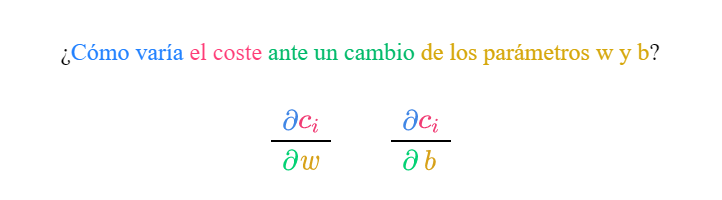
\includegraphics[width=13cm]{images/state-of-art/gradient-descent/dx.png}
    \caption{Derivadas parciales usadas en el descenso del gradiente.}
    \label{fig:gradient_descent}
\end{figure}

\end{itemize}


